\section{Breakdown}

\subsection{Rationale}

	Aim 1 is centered around the creation and modeling of the TCP material. There are multiple methods used to make this process consistent and reliable. Most notably those described in \cite{wu_compact_2017}, where the TCP actuation method is used to manipulate a humanoid hand. With the purpose of simplfication of the creation/modeling process, a precursor fiber with similar specifications to that of the aforementioned article will be purchased.

	In order to achieve a consistent fabrication process, the TCP will be spun using an automated system; similar to that of a rope making machine. The system will be configurable to a set number of rotations, and a set RPM speed, as well as having connections for an adjustable counter-weight which will be used as the third and final configuration input when making the material. Once the fabrication process is created and checked for consistency, data will be collected on the actuation capabilities of the string with varying configuration inputs. A setup will be chosen based on the data collected.

	The next step is to derive a control model formula which can represent the tension exhibited by a single strand of the TCP with inputs of current $[Amps]$ and over a predetermined length of time $[seconds]$. The constant parameters of the system will ideally be the same as the parameters used when creating the TCP string, but will require more testing to legitimize. Because TCP is actuated via heat generation, the system dynamics will be time-dependent, and will be discussed in the next section.

	Finally, a controller will be implemented (figure \ref{fig:control_diagram}), ideally using the aforementioned model formula. The current plan is to utilize an optimal control policy with the inclusion of an accurate model. In cases where the model cannot be applied, a simpler sub-optimal policy may be used instead. Both options are feasible. Model predictive control (MPC) will be considered because of its ability to look into future states, and accurately account for time-dependent variables when given a reliable and accurate model and cost function.

	\begin{figure}[ht]
		\centering
		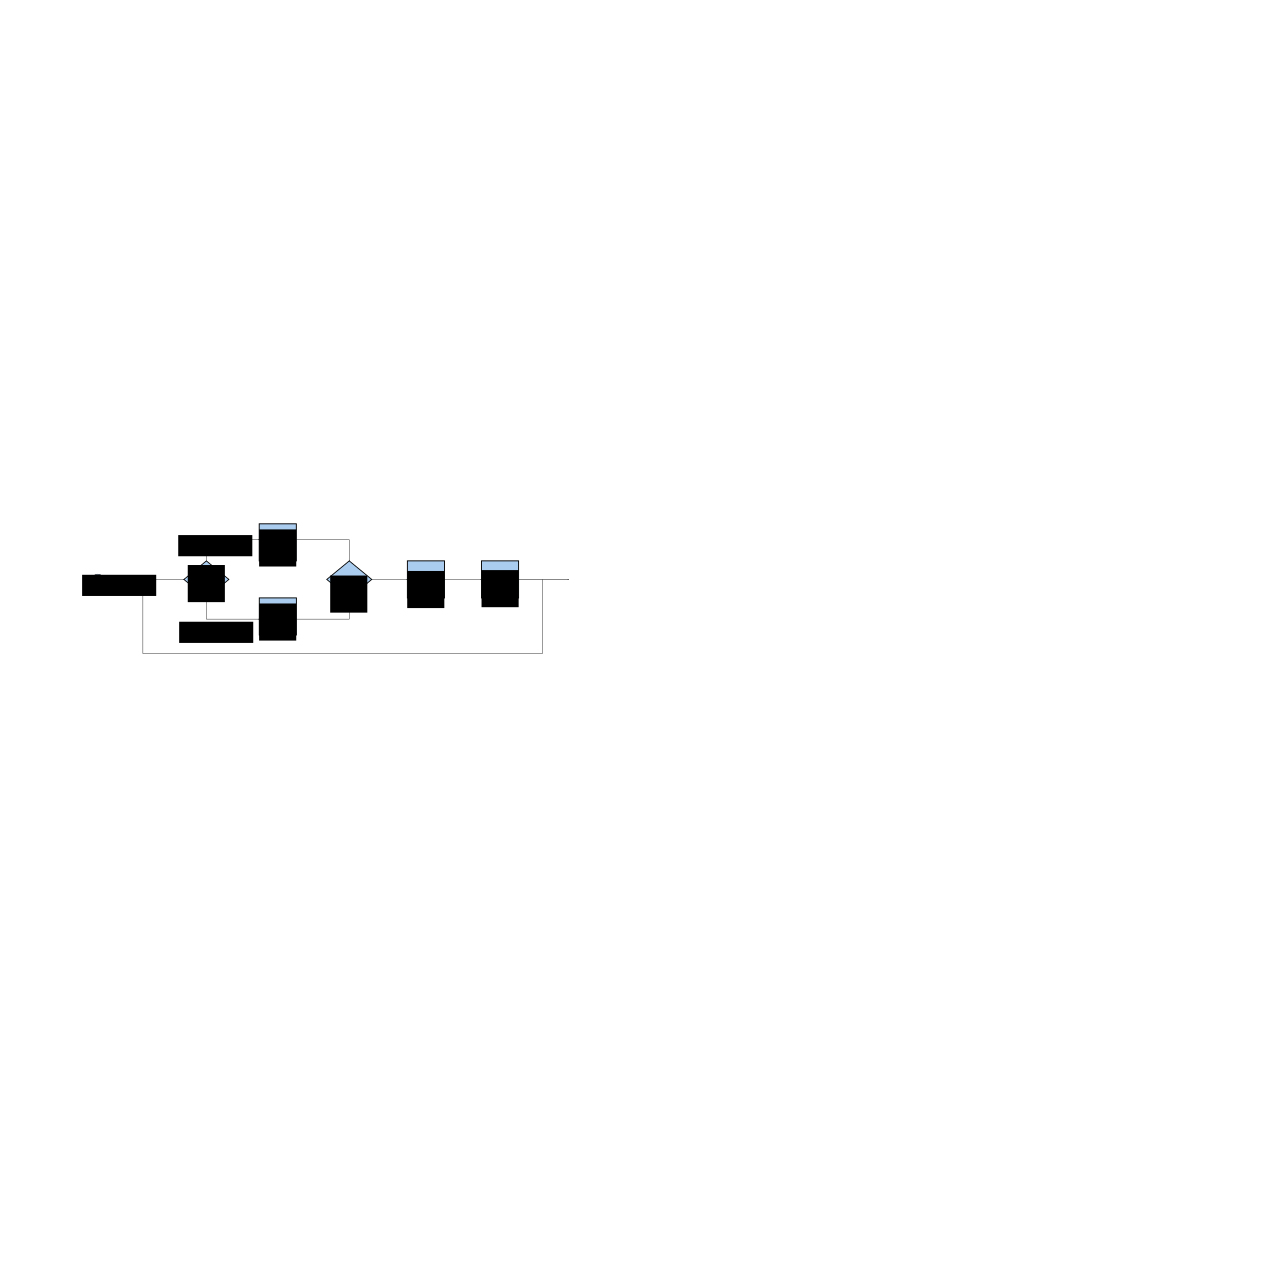
\includegraphics[scale=0.30]{control_diagram}
		\caption{AEI System Control Diagram}
		\label{fig:control_diagram}
	\end{figure}

	Figure \ref{fig:control_diagram} shows the planned controller structure. The user-input block is a set of parameters received from the user during runtime. This will tell the device whether the user is in manual or automated operation modes, and will split into two similarly structured decision branches. With a desired trjectory chosen, the tracking controller will decide the necessary current value before uploading the results to the system dynamics and continuing.

\subsection{Approach}

	\subsubsection{Timeline}

		The fabrication of the TCP material will be facilitated through a modular and controllable stepper motor circuit. The wire of choice will be silver-coated nylon 6/6 precursor fiber, similar to that used in the initial prototype. The control board used for TCP creation will be an Arduino Uno, and will be used to control the RPM of the machine, as well as the total number of spins. The counter-weight attached to the machine can also be adjusted for further variations, but will likely follow similar mechanics to those used in \cite{wu_compact_2017, haines_new_2016, saharan_novel_2019}. For consistency, the length of the TCP created during a given test will be held constant, and will be heat-treated and trained using the research verified by \cite{wu_compact_2017, haines_new_2016}. The fabrication process is currently designated about $25\%$ of total project time. That is, if the project spans a single year, the fabrication process would be given $3[months]$. The bulk of this time period will be spent creating new material and collecting the data points outlined in Section \ref{sect:aim1_modeling_techniques}.
	
		Modeling of the TCP actuation will be completed in parallel to Aims 2 and 3, and will be appointed about $40\%$ of the Aim 1 project schedule, meaning for a year-long project modeling wil be given approximately $4.5[months]$. The system of equations discussed in Section \ref{sect:aim1_modeling_techniques} from \cite{wu_compact_2017} make the assumption that the load place on the TCP is constant. For the purpose of implementation with the AEI system, this assumption cannot be made. The purpose of this portion of the project will be to implement a variable load into the system of equations, as well as merge the system with the continuum robot modeling techniques used in \cite{rao_how_2021}. It should also be noted that some of this period will also be inevitably spent creating more TCP for the testing process.

		The controller for the system will ideally be model-dependent. It is understood that model-dependent controllers, when accurately tuned, can create optimal systems and are more reliable and robust then model-independent alternatives. Considering the time-dependence of the TCP system variables, the use of model predictive control (MPC) will be considered because of its ability to look into future states and solve for the optimal set of inputs at a given point in time. MPC is a control method commonly used in the robotics community for like-wise scenarios and has proven to be one of the most ideal control policies in the field. That said, there are other similarly effective model-independent controller alternatives in the event that an optimal policy is not able to be constructed. Because of the importance of this portion of the project, it will similarly be allocated $40\%$ of the total project time.
		
		The completed timeline, as well as those constructed for Aim 2 and 3, is shown in Figure \ref{fig:full_timeline}.

	\subsubsection{Modeling Techniques}
	\label{sect:aim1_modeling_techniques}
	
		The following section describes the steps taken for TCP modeling as derived in \textit{Modeling of twisted and coiled polymers (TCP) muscle based on phenomenological approach} by Farzad Karami and Yonas Tadesse. The following equations are used to approximate the temperature and displacement of the material based on a given current $[A]$, load $[N]$ and string dimensions.

		The change in resistance with respect to temperature is shown in Equation \ref{eq:tcp_resistance} below.
	
		\begin{equation}
		\label{eq:tcp_resistance}
			R(T) = R_{0} (1 + \alpha (T - T_{0}))
		\end{equation}
	
		Where $R(T)$ represents the current resistance in $[ohms]$, $R_{0}$ is the resistance at a reference temperature, $T_{0}$, and $T$ is the current temperature of the TCP. $\alpha$ is the coefficient of resistivity which is defined more accurately in \cite{yang_top-down_2016} and is closely realted to the coefficient of thermal expansion (CTE). For the purpose of manipulating tension using the TCP mechanics, a material with a negative CTE was chosen. It is further explored that the elastic modulus, E, is also determined by temperature.
	
		For equation \ref{eq:tcp_resistance} to be used accurately during modeling the change in temperature must also be approximated. This is completed below.
	
		\begin{equation}
		\label{eq:tcp_temperature}
			T - T_{\infty} =
				- \frac{R_{0} i^{2}}{-h A + R_{0} i_{2} \alpha}
				\left(
					1 -
					\exp^{\frac{-h A + R_{0} i_{2} \alpha}{m c_{p}}} t
				\right)
		\end{equation}
	
		Where $T_{\infty}$ is the ambient temperature, $i$ is the operating current, $h$ is the coefficient of heat convection, $A$ is the exposed TCP surface area, $m$ is the TCP mass, $c_{p}$ is the specific heat capacity, and $t$ is the time-passed. This is used to approximate the temperature, $T$, of the TCP with respect to a given current, $i$, and time, $t$.
	
		Using Equation \ref{eq:tcp_temperature} in combination with the function for $E$ (equation \ref{eq:tcp_elastic_modulus} and along with the dimensions of the TCP material, the displacement of the TCP can be calculated using the set of equations shown below.
	
		\begin{equation}
		\label{eq:tcp_elastic_modulus}
			E(T) = a_{1} T^{a_{2}} + a_{3}
		\end{equation}
	
		\begin{equation}
		\label{eq:tcp_displacement_elastic}
			\Delta_{el} = \frac{F}{k}
		\end{equation}
		
		\begin{equation}
		\label{eq:tcp_displacement_thermal}
			\Delta_{th} = \delta H
			\begin{matrix}			
				= \frac{L \delta L - \pi D \delta D}{\sqrt{L^{2} - \pi D^{2}}} \\
				= \frac{L^{2}_{0}}{H_{0}} \alpha_{L} (T - T_{0}) - \frac{pi D^{2}_{0}}{H_{0}} \alpha_{T} (T - T_{0})
			\end{matrix}
		\end{equation}
		
		\begin{equation}
		\label{eq:tcp_displacement}
			\Delta H = H_{0} - \Delta_{th} + \Delta_{el}
		\end{equation}
		
		Equation \ref{eq:tcp_elastic_modulus} represents a fitted function for the elastic modulus of a single string of TCP at a given temperature. Equation \ref{eq:tcp_displacement_elastic} is the displacement of the TCP with respect to the load and equation \ref{eq:tcp_displacement_thermal} is the displacement based on the CTE and heat generation via electrical current. Finally, (\ref{eq:tcp_displacement}) is the sum of all displacement methods highlighted in the previous two equations.
	
		Here, $a_{1}$, $a_{2}$ and $a_{3}$ are the fitted curve coefficients, $F$ is the load on the TCP, $k$ is the elastic coefficient (not derived here), $L_{0}$ is the initial TCP stretched length, $H_{0}$ is the initial TCP coiled length, $D_{0}$ is the diameter of the coiled wire, $\alpha_{L}$ is the longitudinal CTE, and $\alpha_{T}$ is the transverse CTE. The suse of these equations allow for the approximation of the TCP length at a given point in time.
	
		The issue that arises here is the assumption that the load, $F$, is constant. For the purpose of implementation in AEI, the tension must be dynamic in the modeling. This issue will be addressed during the modeling 

	\subsubsection{Experimental Process}
	\label{sect:aim1_experimental_process}
	
		Verifying the controller system will be completed parallel to its programming. Once the fabrication method for the TCP is finalized, a few weeks will be designated to creating TCP and collecting data over its behavior when supplied with varying levels of current, constant counterweight magnitudes and with differing ply-numbers. The collected data points will include, but will not be limited to, TCP temperature, displacement and resistance trends. In the schedule shown in Figure \ref{fig:full_timeline} these tasks are represented by items 1-8.
		
		With the load-static model verified, the system of equations will either be adjusted for variable load, or a method of numerically approximating the tension in the TCP will be implemented. The goal of this step will be to create a conversion from current TCP temperature to string tension. Modeling for tension will allow the researcher to design a single-strand controller which is capable of holding a desired displacement by manipulating the tension in the TCP wires. The items span 9-13 in the comprehensive schedule (Figure \ref{fig:full_timeline}).
		
		With this, the system can be expanded to continuum robot modeling using the piecewise constant-curvature method, better explained in \cite{rao_how_2021}. The controller can also be expanded to 3-D continuum robot actuation by similarly manipulating current to control deflection via the tension in the TCP (schedule items 15-21).
		
		At this step, the internal position sensing system will be addressed and there are multiple options available on the market. The intent with this component is to understand in real-time the position of the end effector, and compare to the model. These include electromagnetic sensing, explained thoroughly in \cite{guo_continuum_2019}, and optical sensing. Preliminary research suggests the former will be more viable for the purpose of the device and to the hospital environment.

\subsection{Risks and Alternatives}

	It is understood that all of the steps taken in this portion of the development process are subject to considerable obstacles. That said, each of the discussed approaches have alternative methods of attack which should still achieve the overarching goals of the research.

	In the case of fabrication, there are multiple methods for twisting, annealing, and training the TCP wires. This process is well documented in the aforementioned articles and is unlikely to be problematic, but if the creation process does not work as intended, there are many alternatives to twisting the string and prepping it for annealing and training. The TCP essentially requires a small-scale rope-making machine, and thus has many vehicles for a consistent system.
	
	While methods of modeling the TCP behavior have been discussed, and are proven to be reliable, there is still a chance that a comprehensive model of the TCP will not be as easily generated as predicted. In the event that a model-based optimal controller cannot be constructed accurately, it is also possible to train a model-free neural network to produce the intended controller behavior. This would involve considerably more data on configuration details, but is very possible and has been done for likewise projects in the past \cite{yang_efficient_2000, byravan_se3-nets_2017}.